\documentclass[english]{psi_easy}

%% Language and font encodings
\usepackage[english]{babel}
\usepackage[utf8x]{inputenc}
\usepackage[T1]{fontenc}
\usepackage{comment} 

%% Useful packages
\usepackage{amsmath}
\usepackage{graphicx}
\usepackage[table,xcdraw]{xcolor}
\usepackage{booktabs}
% \usepackage[colorinlistoftodos]{todonotes}
\usepackage[colorlinks=true, allcolors=blue]{hyperref}

% float placement
\usepackage{float}

% cable color bullets
\usepackage{tikz}

% for trademark sign 'circledR'
\usepackage{amssymb}

% for PSI logo on Rolfs title page
\usepackage{epsfig}

%% Set title here for EASY title page
\PsiEasyTitle{Guideline: Device cables and connectors for \EtherCAT{} motion control and simple IO}

% ---- custom commands
% Schneidersche Einrueckung in 'itemize'
\newcommand{\itemIndent}[2]{{\makebox[3cm]{#1:\hfill} #2.}}
% draw colored circle
\newcommand{\wireColor}[1]{\tikz\draw[black,fill=#1] (0,0) circle (.9ex); #1}
\newcommand{\EtherCAT}[0]{EtherCAT$^{\tiny{\circledR}}$}
% ---- custom commands end

%% Document begins here
\begin{document}

%
% --- Title page by R. Follath
% comment the next line for EASY export, as the cover page is handled by the system
\input 0_titlePage

% set page counter to '2', as easy will create the cover page and need the PDF for import to start on page 2.
\clearpage
\setcounter{page}{2}

%% TOC
\tableofcontents

%% Abstract
\begin{abstract}
This guideline summarizes the requirements for cable and connector selection as well as routing for SLS~2.0 and all new installations in other facilities of PSI utilizing \EtherCAT{} based motion control and simple IO.
The guideline will define strict requirements, indicated by the word ‘\textbf{must}’ or ‘\textbf{mandatory}’, as well as strong suggestions indicated by the word ‘\textbf{should}’.
Weak requirements are indicated by the word ‘\textbf{preferred}’.
This guideline describes devices operated in air, under normal environmental conditions (298~K (25~$^\circ$C), 1013~mbar, 50~\%~rH) no or low radiation.
Exceptions apply for devices operated in any other environments including, but not limited to, vacuum, low temperature, strong magnetic fields or high radiation.
Common exceptions are described in the respective sections.
\end{abstract}

%% Actual Text
\section{General Rules}

\subsection{Patching}
% This paragraph describes the signal path from the actuator/sensor to the controller.
% The signal path can comprise various patch panels.
% This includes \emph{(a)}~a device patch panels\footnote{Suppliers are only required to deliver device patch panels. Subsequent patching is handled at PSI.}, \emph{(b)}~an optional intermediate patch panel and \emph{(c)}~a mandatory controller patch panel.
% Depending on the size, complexity multiple device patch panels are allowed.
% Requirements for the patch panels are given below:
\begin{itemize}
    \item A device patch panel is mandatory.
    \item For larger devices, multiple device patch panels are allowed.
    The placement should allow easy access during operation. 
    The placement is subject to discussion during the design phase and has to be approved by PSI during the final design review (FDR).
    \item If the manufacturer prefers to supply a cabinet or other enclosure to handle the signal distribution, this is subject of approval by PSI.
            In this case the internal routing has to account for signal cross talk.
            The outside connection must meet the requirements of the device patch panel. 
    \item Male connectors must be used on the device patch panel.
    % \item Female connectors must be used on the controller patch panel.
    \item Patch panel feedthroughs must be placed with at least 30~mm spacing center to center.
            The orientation must comply with Fig.~\ref{fig:PanelCutOut} to allow interference free connection of angled connectors.
\end{itemize}

\begin{figure}[H]
\centering
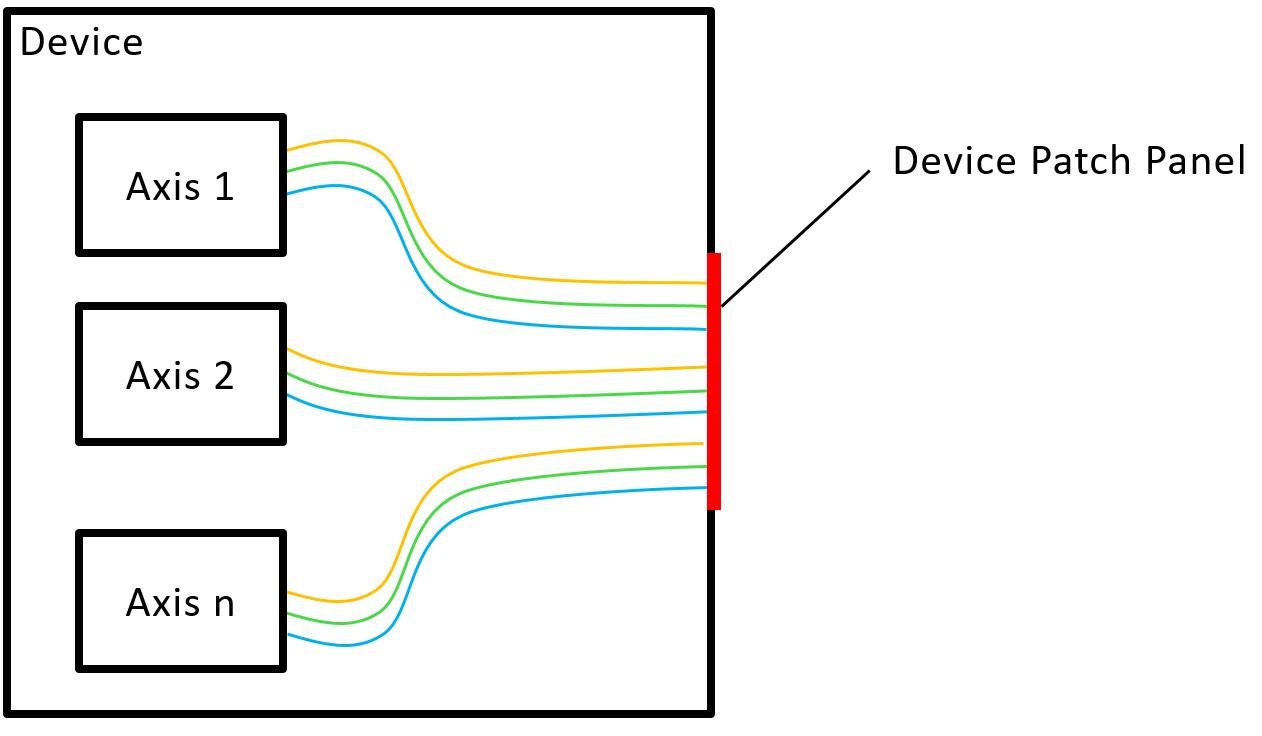
\includegraphics[width=0.4\textwidth]{Figures/DevicePatchPanel.jpg}
\caption{\label{fig:DevicePatchPanel}Overview, device and patch panel}
\end{figure}


Routing from the source to the patch panel can be achieved by two options (Fig.~\ref{fig:PatchingOptions}).
\begin{itemize}
    \item[\bf A] Direct connection of the cable to the panel feedthrough, e.g. by utilizing the part \emph{Harting, 21 03 821 1525 (4, 5-pole), 21 03 821 1825 (8-pole)}
    \item[\bf B] Use of a pre-manufatured extension cabel in conjunction with a corresponding M12 feedthrough. The part \emph{Murr Elctronic, 7000-42111 (4,5-pole), 7000-48111 (8-pole), } can be used for this option.
\end{itemize}
Both options are allowed, whereas option A is preferred, as it is more compact.
In the subsequent example depictions, only option A is used for simplicity.

\begin{figure}[H]
\centering
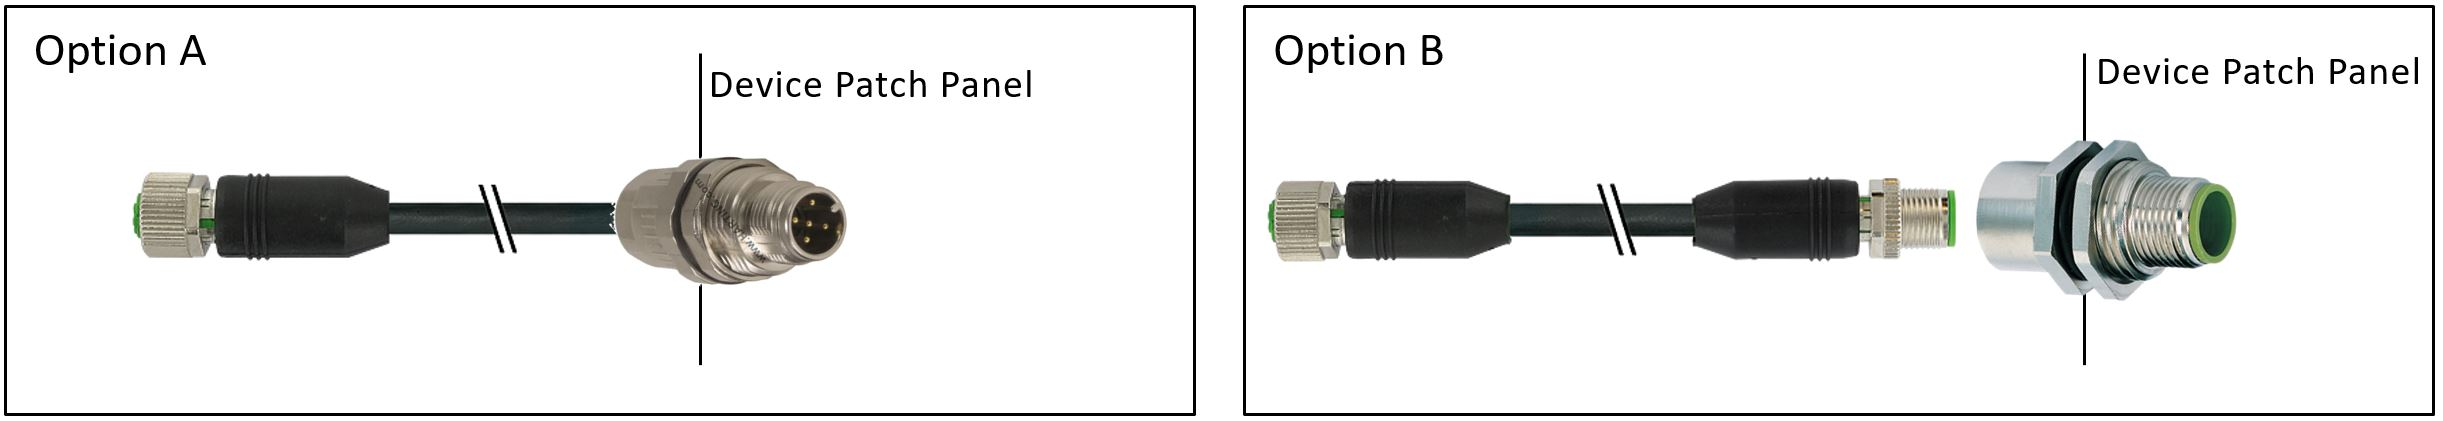
\includegraphics[width=0.9\textwidth]{Figures/PatchingOptions.jpg}
\caption{\label{fig:PatchingOptions}Two different approaches for patch panel design}
\end{figure}


\begin{figure}[H]
\centering
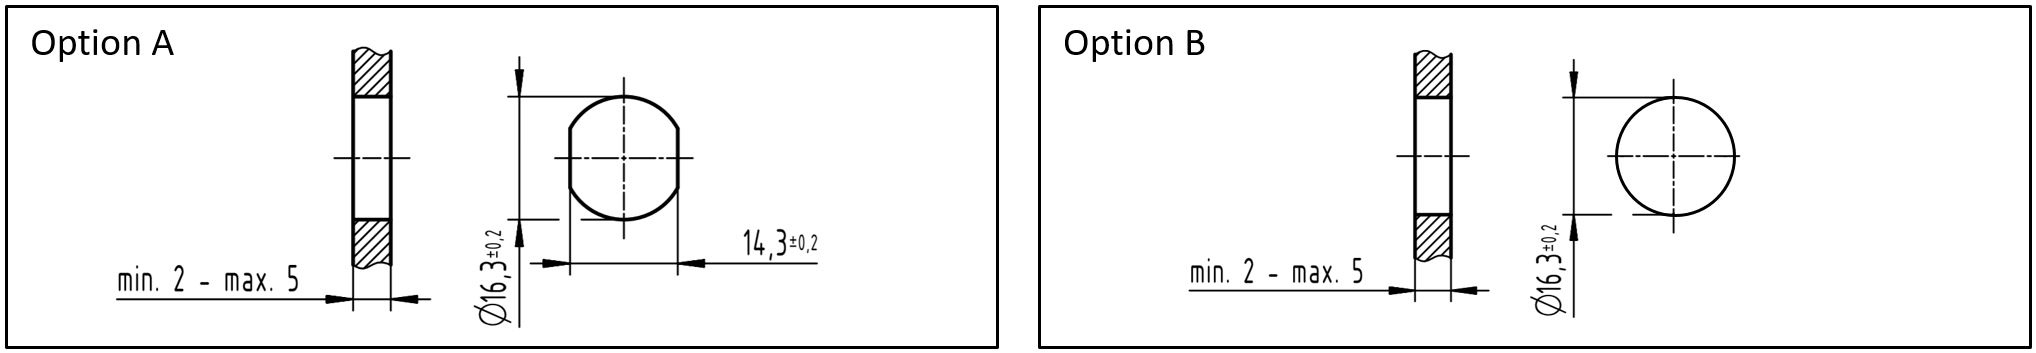
\includegraphics[width=0.9\textwidth]{Figures/PanelCutOut.jpg}
\caption{\label{fig:PanelCutOut}Panel cutouts for Option A and B}
\end{figure}

\subsection{Degree of Protection}
Connectors must be encapsulated or protected from direct access/touch. At minimum IP2X according to IEC standard 60529 must be met.

\subsection{Routing}
\begin{itemize}
    \item A strain relief of all cables is mandatory.
    \item The minimum bending radius of all cables must be obeyed.
    \item Moving components should feature a drag chain or other mechanical feature to ensure clean and repeatable guiding of cables.
    \item The cable length from actor/sensor to device patch panel must be limited to a maximum of 5~m.
\end{itemize}

\subsection{Shielding}
\begin{itemize}
    \item All cables and connectors must be shielded.
\end{itemize}

\subsection{Protective Earth (PE)}
\begin{itemize}
    \item The patch panel must be electrically connected to PE star point with sufficient cross section.
\end{itemize}

\subsection{Documentation}
\begin{itemize}
    \item A wiring diagram with all connectors and cables must be provided.
    \item All connectors and cables must be labeled according to the wiring diagram.
    \item The BOM\footnote{bill of materials} of the CAD assembly should indicate the utilized connector type, vendor and part number. Alternatively, a separate list of components must be provided.
\end{itemize}

\section{Connectors and Cables}

In this section, the connector types as well as the pinouts are defined.
Any deviation for the subsequently listed requirements must be approved by PSI prior to the FDR.
Exception: For devices operated in vacuum- or other vessels with feedthroughs, a direct cable routing from the respective feedthrough to the patch panel must be realized.
The feedthroughs should not share signals with potential cross talk, i.e. motor and thermocouple.
The selection of the feedthrough is subject of the manufacturer, except for thermocouples.
The latter have to approved by PSI individually deepening on application.

\subsection{Connector overview (Device Patch Panel)}

An overview of the connectors with pinouts for their various applications is given in table~\ref{tab:connectorOverview}.

\begin{table}[!htb]
\caption{\label{tab:connectorOverview}Connector overview.}
\begin{minipage}{\linewidth}
\centering
\begin{tabular}{|c|c|c|c|c|c|c|}
\hline
\textbf{}                         & \textbf{Stepper} & \textbf{Encoder} & \textbf{Limits} & \textbf{Pt-100} & \textbf{TC}\footnote{thermocouple} & \textbf{Requirement} \\ \hline
\textbf{Connector type}           & \multicolumn{5}{c|}{M12}                                                              & must                 \\ \hline
\textbf{Coding}                   & \multicolumn{5}{c|}{A}                                                                & must                 \\ \hline
\textbf{Contacts}                 & 4                & 8                & 5               & 5               & 5           & must                 \\ \hline
\textbf{Shielding}                & \multicolumn{5}{c|}{yes}                                                              & must                 \\ \hline
\textbf{Norm}                     & \multicolumn{5}{c|}{IEC 61076-2-101}                                                   & must                 \\ \hline
\textbf{Connector locking system} & \multicolumn{5}{c|}{Crimp}                                                            & should               \\ \hline
\end{tabular}
\end{minipage}
\end{table}

\subsection{Stepper motors}
Only Beckhoff cables should be used due to the larger conductor cross section, compared to standard M12 cables.
Alternatively, custom manufactured cables with sufficient cross section can be used.

\begin{table}[H]
\centering
\caption{\label{tab:stepperPinout}Pinout of stepper motor connector.}
\begin{tabular}{@{}p{1cm}p{4cm}p{4cm}@{}}
\toprule
Pin & Signal & Color             \\ \midrule
1   & A      & \wireColor{brown} \\ \midrule
2   & A/     & \wireColor{white} \\ \midrule
3   & B      & \wireColor{blue}  \\ \midrule
4   & B/     & \wireColor{black} \\ \bottomrule
\end{tabular}
\end{table}

\subsubsection{How to connect a Beckhoff AS1000 series stepper}
\begin{figure}[H]
\centering
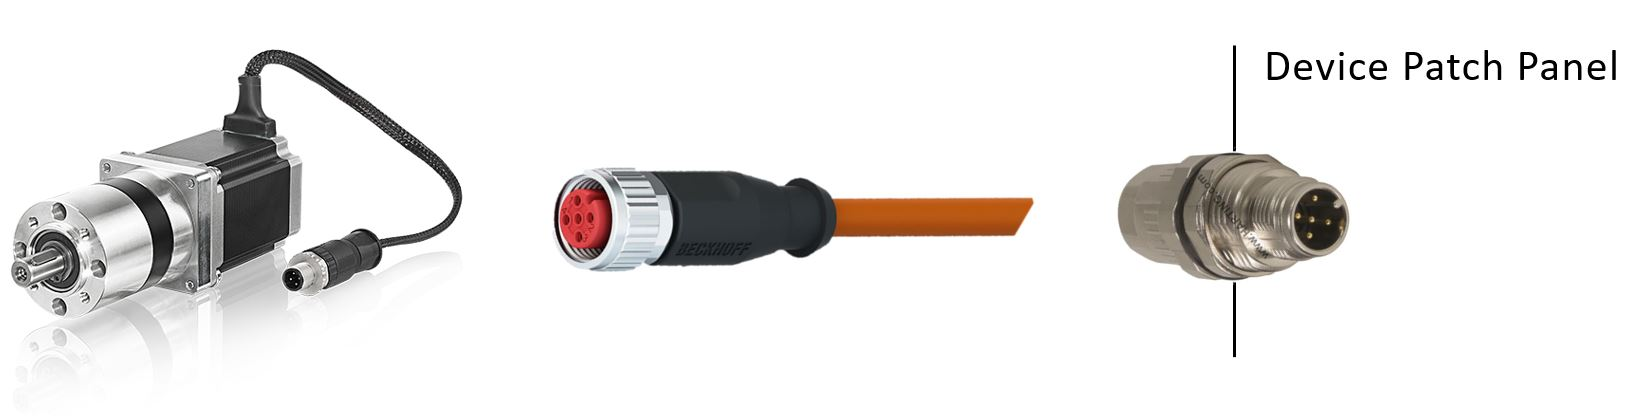
\includegraphics[width=0.7\textwidth]{Figures/StepperAS1000.jpg}
\caption{\label{fig:StepperAS1000}Example wiring for AS1000 series motor.}
\end{figure}

\begin{itemize}
    \item \itemIndent{Motor}{Beckhoff, AS1000 Series (comes with assembled M12 connector)}
    \item \itemIndent{Cable}{Beckhoff, ZK4000-6200-2xxx}
    \item \itemIndent{Feedthrough}{Harting, 21 03 821 1525}
\end{itemize}

\subsubsection{How to connect a Beckhoff AS2000 series stepper}
\begin{figure}[H]
\centering
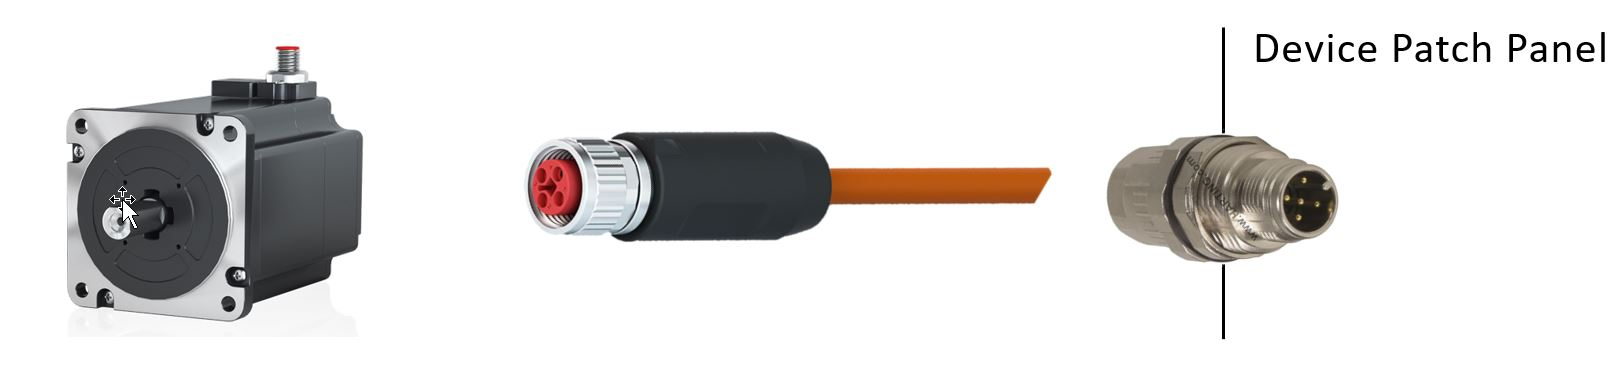
\includegraphics[width=0.7\textwidth]{Figures/StepperAS2000.jpg}
\caption{\label{fig:StepperAS2000}Example wiring for AS2000 series motor.}
\end{figure}

\begin{itemize}
    \item \itemIndent{Motor}{Beckhoff, AS2000 Series (M12, T-coded, connector on motor)}
    \item \itemIndent{Cable}{Beckhoff, ZK4000-7700-0xxx}
    \item \itemIndent{Feedthrough}{Harting, 21 03 821 1525}
\end{itemize}

\subsubsection{How to connect a motor with flying leads}
\begin{figure}[H]
\centering
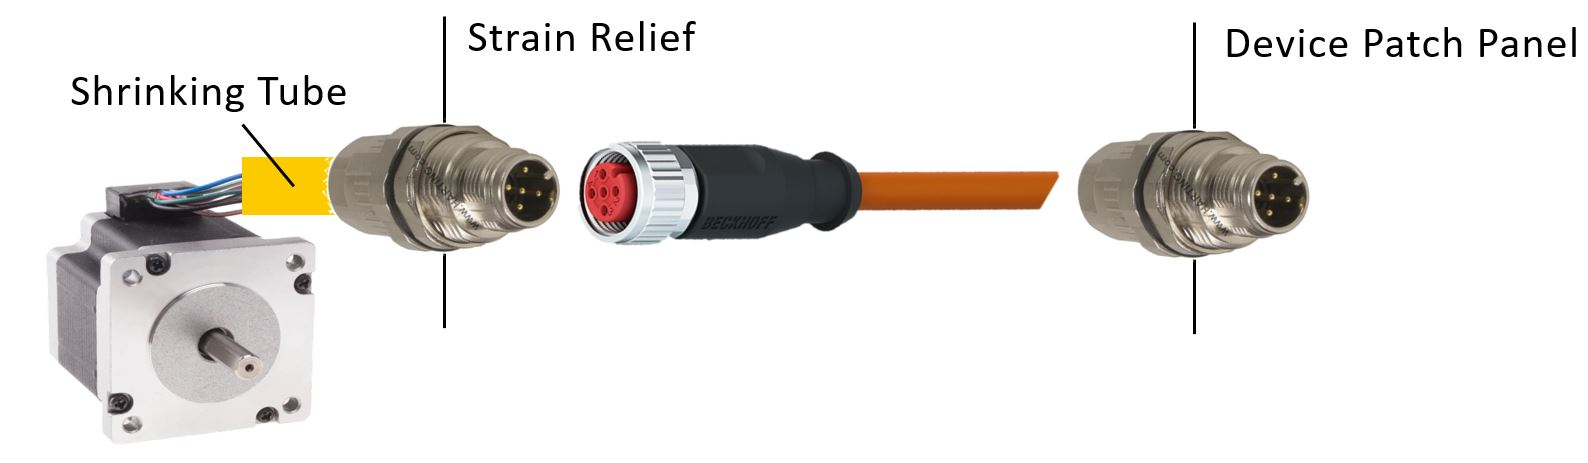
\includegraphics[width=0.7\textwidth]{Figures/StepperFlyingLeads.jpg}
\caption{\label{fig:StepperFlyingLeads}Example wiring for stepper with flying leads.}
\end{figure}

\begin{itemize}
    \item \itemIndent{Motor}{Any manufacturer\footnote{For motors with up to 5~A peak phase current. For higher current, please contact the project owner.}}
    \item \itemIndent{Cable}{Beckhoff, ZK4000-6200-2xxx}
    \item \itemIndent{Feedthrough}{Harting, 21 03 821 1525}
\end{itemize}

\subsection{Encoders}
All encoders must be absolute. The information length should be restricted to 26 bit for linear encoders or 12/13 bit for multi turn rotary encoders. Higher information length has to be approved by PSI. Any other encoder type also has to be approved by PSI with a detailed description why the afore defined requirements cannot be met.

\begin{table}[H]
\centering
\caption{\label{tab:encoderPinout}Pinout of encoder connector.}
\begin{tabular}{@{}p{1cm}p{4cm}p{4cm}p{4cm}@{}}
\toprule
Pin & Signal BiSS-C & Signal SSI & Color        \\ \midrule
1   & 0~V   & 0~V       & \wireColor{white}   \\ \midrule
2   & V~$+$   & V~$+$       & \wireColor{brown}   \\ \midrule
3   & MA~$+$  & Clock~$+$   & \wireColor{green}   \\ \midrule
4   & MA~$-$  & Clock~$-$   & \wireColor{yellow}  \\ \midrule
5   & SLO~$+$ & Data~$+$    & \wireColor{gray}  \\ \midrule
6   & SLO~$-$ & Data~$-$    & \wireColor{pink}  \\ \midrule
7   & Set   & Set       & \wireColor{blue}  \\ \midrule
8   & Direction  & Direction  & \wireColor{red}  \\ \bottomrule
\end{tabular}
\end{table}

\subsubsection{How to connect an Encoder with matching pin assignment (1:1)}
\begin{figure}[H]
\centering
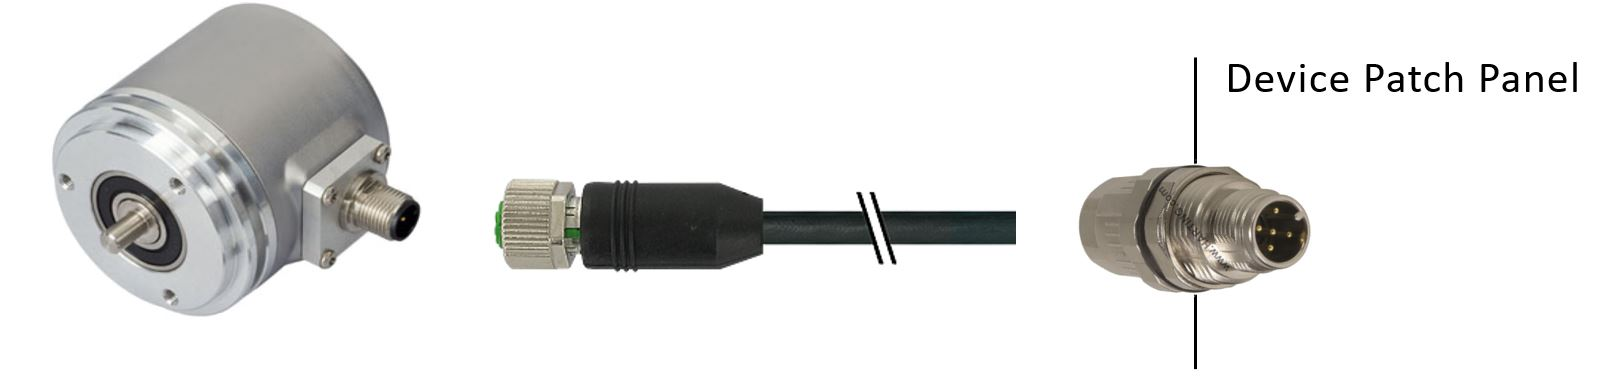
\includegraphics[width=0.7\textwidth]{Figures/Encoder1to1pinout.jpg}
\caption{\label{fig:Encoder1to1pinout}Example wiring for Encoder with matching pin assignment.}
\end{figure}

\begin{itemize}
    \item \itemIndent{Encoder}{Any manufacturer}
    \item \itemIndent{Cable}{Phoenix Contact, 1522888}
    \item \itemIndent{Feedthrough}{Harting, 21 03 821 1825}
\end{itemize}

\subsubsection{How to connect an Encoder with non-matching pin assignment}
\begin{figure}[H]
\centering
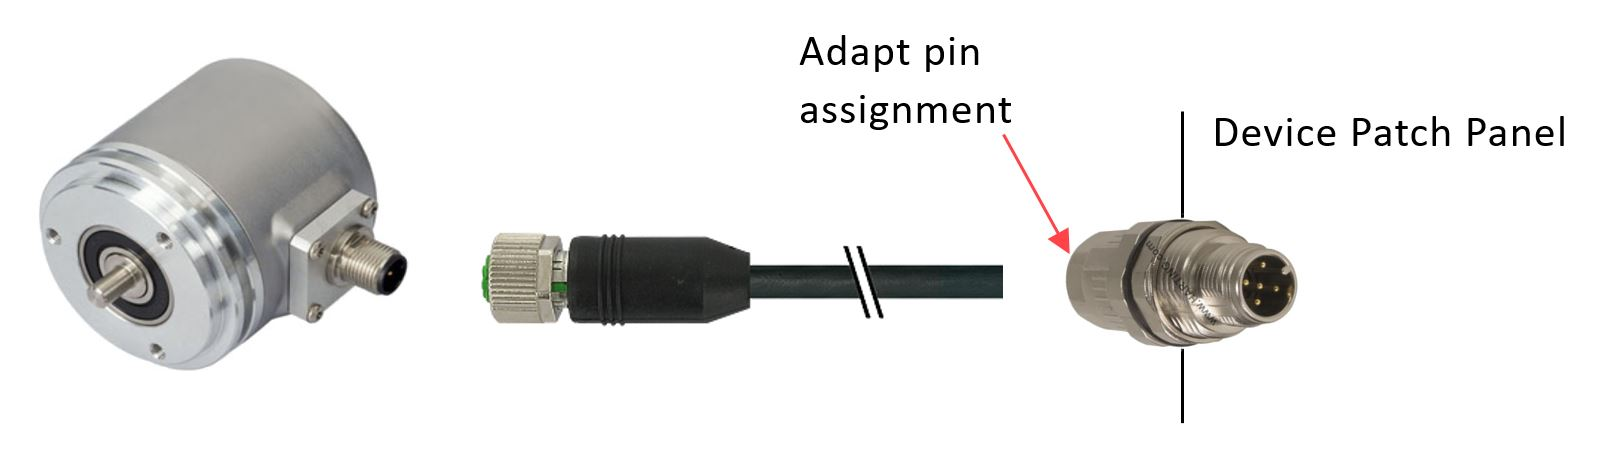
\includegraphics[width=0.7\textwidth]{Figures/EncoderPinoutAdaption.jpg}
\caption{\label{fig:EncoderPinoutAdaption}Example wiring for Encoder with non-matching pin assignment.}
\end{figure}

\begin{itemize}
    \item \itemIndent{Encoder}{Any manufacturer}
    \item \itemIndent{Cable}{Any manufacturer}
    \item \itemIndent{Feedthrough}{Harting, 21 03 821 1825}
\end{itemize}


\subsection{Limit switches/sensors}
All limit switches must be tolerant to 24 VDC. Active sensors must be of PNP type. Mechanical switches must be normally closed (NC). Any deviation from those requirements have to be approved by PSI. Negative (backward) and positive (forward) limit switches should be connected to one connector. Use a T- or Y –splitter to split the signal for the individual switches. The use of M8 switches is preferred, M12 is allowed, flying leads should be avoided.

\subsubsection{Pin assignment for limit switches (on device patch panel)}

\begin{table}[H]
\centering
\caption{\label{tab:LSPatchPanel}Pin assignment for limit switches (patch panel).}
\begin{tabular}{@{}p{1cm}p{4cm}p{4cm}@{}}
\toprule
Pin & Signal & Color\\ \midrule
1   & V~$+$                   & \wireColor{brown} \\ \midrule
2   & Negative Limit        & \wireColor{white} \\ \midrule
3   & GND                   & \wireColor{black}  \\ \midrule
4   & Positive Limit        & \wireColor{blue} \\ \midrule
5   & Output (e.g.\ brake)  & \wireColor{gray}  \\ \bottomrule
\end{tabular}
\end{table}

\subsubsection{Pin assignment for limit switches (M8 connector)}

\begin{table}[H]
\centering
\caption{\label{tab:LSSensor}Pin assignment for limit switches (M8 connector, DIN EN 61076-2-104).}
\begin{tabular}{@{}p{1cm}p{4cm}p{4cm}@{}}
\toprule
Pin & Signal & Color             \\ \midrule
1   & V~$+$    & \wireColor{brown} \\ \midrule
2   & n.c.\  &  \\ \midrule
3   & GND    & \wireColor{blue}  \\ \midrule
4   & Signal & \wireColor{black} \\ \bottomrule
\end{tabular}
\end{table}

\subsubsection{How to connect sensors with M8 connector}
\begin{figure}[H]
\centering
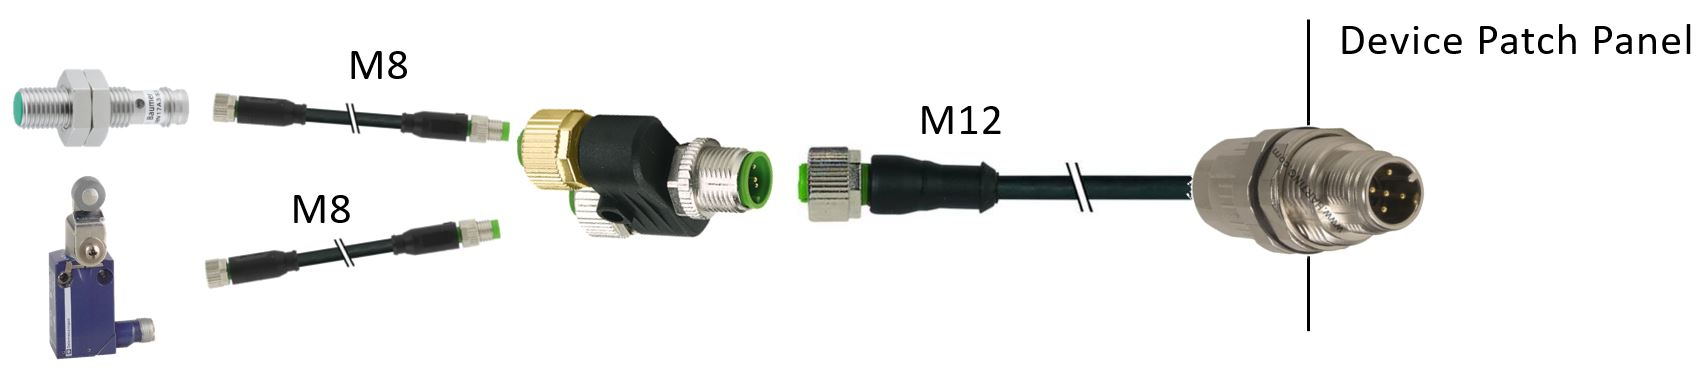
\includegraphics[width=0.7\textwidth]{Figures/LimitSwitchesM8.jpg}
\caption{\label{fig:LimitSwitchesM8}Example wiring for limit sensors with M8 connector and T-splitter.}
\end{figure}

\begin{itemize}
    \item \itemIndent{Limit Switches}{Any manufacturer}
    \item \itemIndent{Cable M8}{Phoenix Contact, 1456310}
    \item \itemIndent{T-splitter}{Murr Electronics, 7000-41201}
    \item \itemIndent{Cable M12}{Phoenix Contact, 1682951}
    \item \itemIndent{Feedthrough}{Harting, 21 03 821 1525}
\end{itemize}

\subsubsection{How to connect sensors with flying leads}
\begin{figure}[H]
\centering
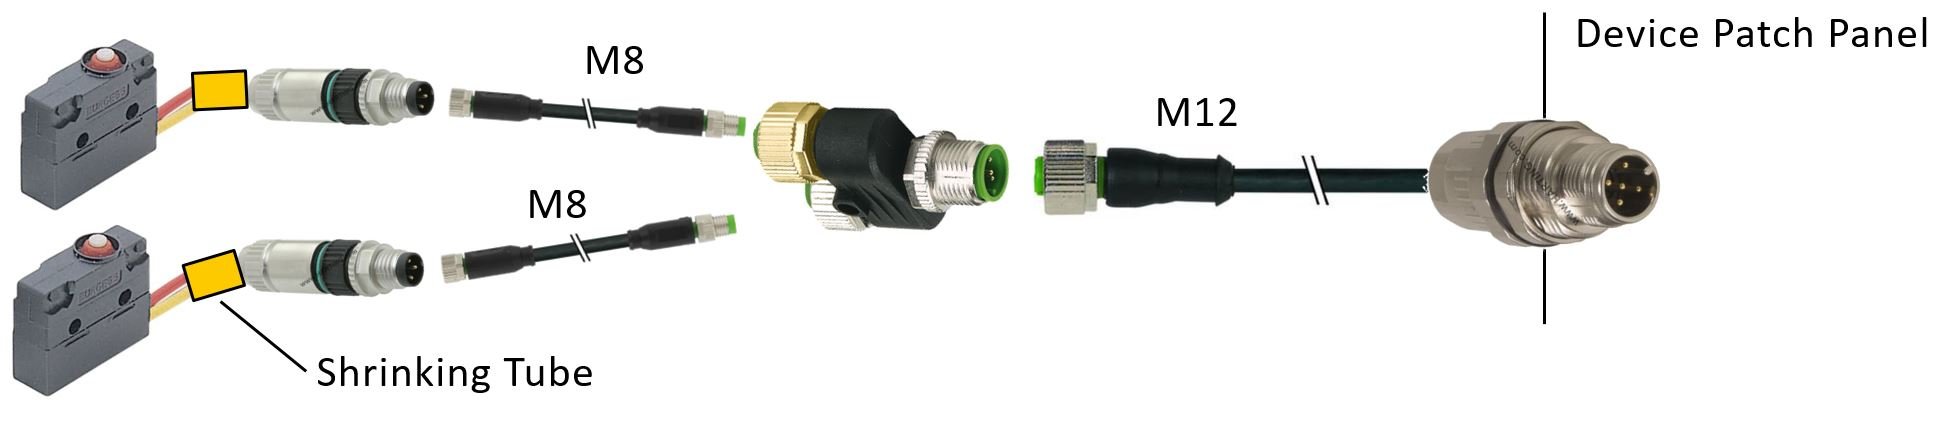
\includegraphics[width=0.7\textwidth]{Figures/LimitSwitchFlyingLeads.jpg}
\caption{\label{fig:LimitSwitchFlyingLeads}Example wiring for limit sensors with flying leads and T-splitter.}
\end{figure}

\begin{itemize}
    \item \itemIndent{Limit Switches}{Any manufacturer}
    \item \itemIndent{Connector N8}{Harting, 21 02 151 1305}
    \item \itemIndent{Cable M8}{Phoenix Contact, 1456310}
    \item \itemIndent{T-splitter}{Murr Electronics, 7000-41201}
    \item \itemIndent{Cable M12}{Phoenix Contact, 1682951}
    \item \itemIndent{Feedthrough}{Harting, 21 03 821 1525}
\end{itemize}

\textbf{Alternatively, use patch box instead of T-Splitter}

\subsection{Temperature measurement}
\subsubsection{Pin assignment for Pt100}

\begin{table}[H]
\centering
\caption{\label{tab:Pt100Pinout}Pin assignment Pt100.}
\begin{tabular}{@{}p{1cm}p{4cm}p{4cm}@{}}
\toprule
Pin & Signal & Color             \\
\midrule
1   & RL~$+$    & \wireColor{brown} \\ \midrule
2   & R~$+$     & \wireColor{white} \\ \midrule
3   & RL~$-$    & \wireColor{black} \\ \midrule
4   & R~$-$     & \wireColor{blue}  \\ \midrule
5   & Shield    & \wireColor{gray}  \\
\bottomrule
\end{tabular}
\end{table}

\begin{figure}[H]
\centering
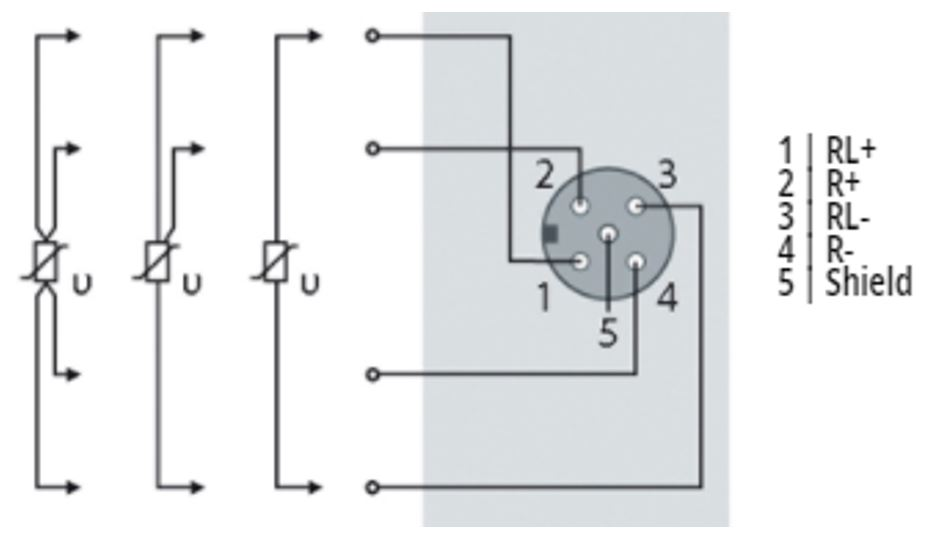
\includegraphics[width=0.4\textwidth]{Figures/Pt100Wiring.jpg}
\caption{\label{fig:Pt100Wiring}Example wiring for Pt100 in different connection methods.}
\end{figure}

\subsubsection{Pin assignment for thermocouples}
For thermocouples only the pinout is defined, conductor color an type can be chosen as needed.

\begin{table}[H]
\centering
\caption{\label{tab:TCPinout}Pin assignment thermocouple.}
\begin{tabular}{@{}p{1cm}p{4cm}p{4cm}@{}}
\toprule
Pin & Signal & Color             \\ \midrule
1   & Compensation A \footnote{Optional: For cold junction compensation (Pt1000 required)}   & free \\ \midrule
2   & Input~$+$           & free \\ \midrule
3   & GND \footnote{Optional: For cold junction compensation (Pt1000 required)}              & free \\ \midrule
4   & Input~$-$           & free  \\ \midrule
5   & Shield            & free  \\ \bottomrule
\end{tabular}
\end{table}

\begin{figure}[H]
\centering
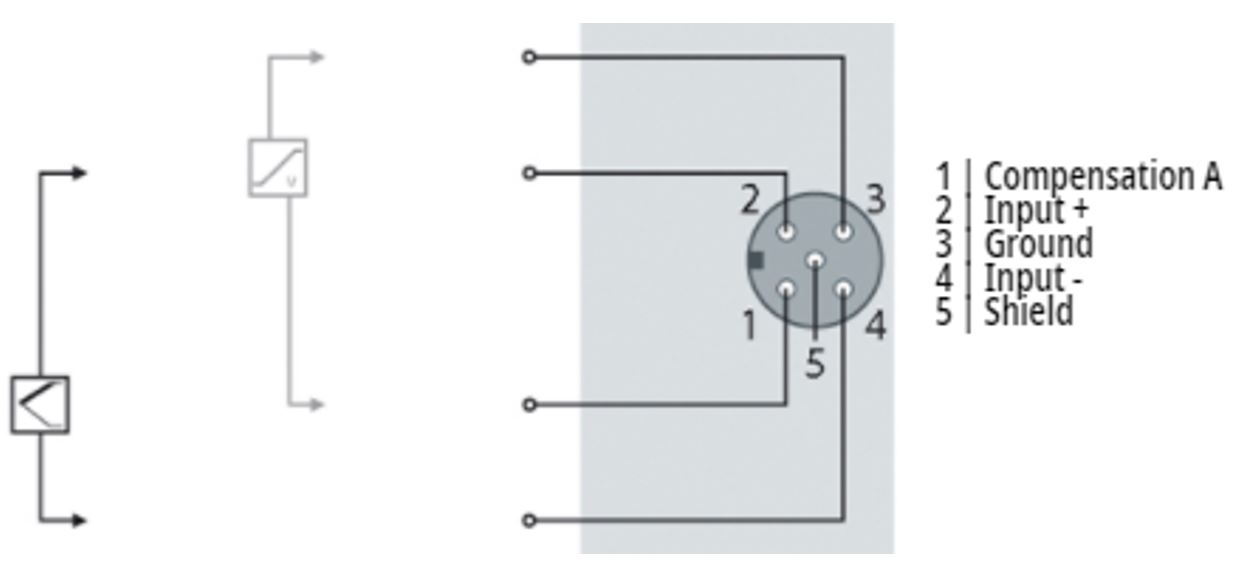
\includegraphics[width=0.5\textwidth]{Figures/ThermocoupleWiring.jpg}
\caption{\label{fig:ThermocoupleWiring}Example wiring for thermocouples.}
\end{figure}


%List of sources
Harting
RS-online (stepper flying leads)
Beckhoff
Posital
Baumer
Saia
Murr
Phoenix Contact

\cite{BeckhoffWeb}
\cite{HartingWeb}



% \subsection{How to add Citations and a References List}

% You can upload a \verb|.bib| file containing your BibTeX entries, created with JabRef; or import your \href{https://www.overleaf.com/blog/184}{Mendeley}, CiteULike or Zotero library as a \verb|.bib| file. You can then cite entries from it, like this: \cite{greenwade93}. Just remember to specify a bibliography style, as well as the filename of the \verb|.bib|.

% You can find a \href{https://www.overleaf.com/help/97-how-to-include-a-bibliography-using-bibtex}{video tutorial here} to learn more about BibTeX.

% We hope you find Overleaf useful, and please let us know if you have any feedback using the help menu --- or use the contact form at \url{https://www.overleaf.com/contact}!

\bibliographystyle{plain}
\bibliography{companies}

\end{document}